\section{Auswertung}
\label{sec:Auswertung}

% Messwerte: Alle gemessenen physikalischen Größen sind übersichtlich darzustellen.

% Auswertung:
% Berechnung der geforderten Endergebnisse
% mit allen Zwischenrechnungen und Fehlerformeln, sodass die Rechnung nachvollziehbar ist.
% Eine kurze Erläuterung der Rechnungen (z.B. verwendete Programme)
% Graphische Darstellung der Ergebnisse

Im Folgenden werden die Messergebnisse aufgelistet und es werden entsprechende Ausgleichsrechnungen ausgeführt.

\subsection{Untersuchung des Lock-In Verstärkers bei verschiedenen Phasenverschiebungen}

In \autoref{fig:1} und \autoref{fig:2} sind die Screenshots des Oszilloskops für die Phasenunterschiede \SIlist{0;45;90;180;270}{\degree} dargestellt.
Hierbei wird die Spannung vor dem Tiefpass abgegriffen, in \autoref{fig:1} der Noise-Generator überbrückt und in \autoref{fig:2} der Noise-Generator zwischengeschaltet. (siehe \autoref{sec:Durchführung})

\begin{figure}
    \centering
    \begin{subfigure}{0.3\textwidth}
        \centering
        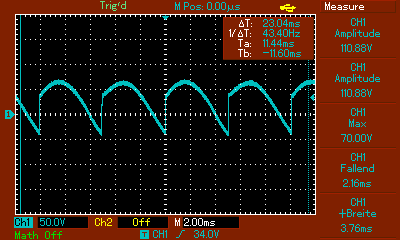
\includegraphics[width=\textwidth]{images/1_0.png}
        \caption{$\varphi = \SI{0}{\degree}$}
        \label{fig:1_0}
    \end{subfigure}
    \begin{subfigure}{0.3\textwidth}
        \centering
        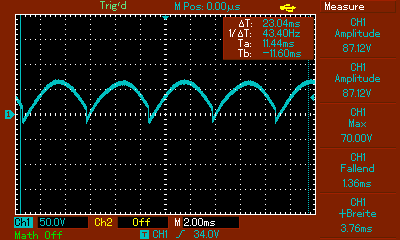
\includegraphics[width=\textwidth]{images/1_45.png}
        \caption{$\varphi = \SI{45}{\degree}$}
        \label{fig:1_45}
    \end{subfigure}
    \begin{subfigure}{0.3\textwidth}
        \centering
        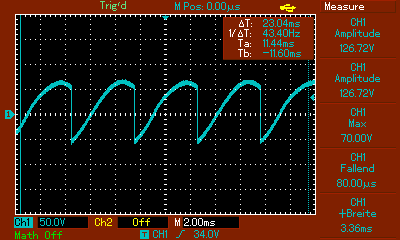
\includegraphics[width=\textwidth]{images/1_90.png}
        \caption{$\varphi = \SI{90}{\degree}$}
        \label{fig:1_90}
    \end{subfigure}
    \par\medskip % Vertikaler Platz
    \begin{subfigure}{0.3\textwidth}
        \centering
        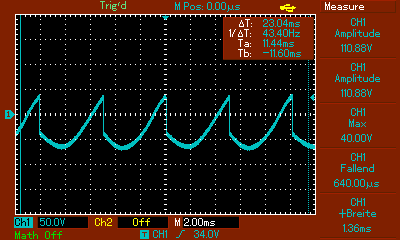
\includegraphics[width=\textwidth]{images/1_180.png}
        \caption{$\varphi = \SI{180}{\degree}$}
        \label{fig:1_180}
    \end{subfigure}
    \begin{subfigure}{0.3\textwidth}
        \centering
        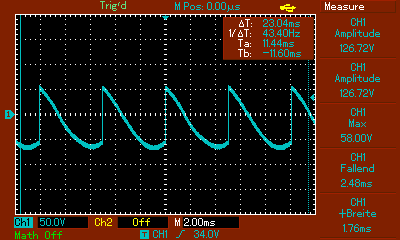
\includegraphics[width=\textwidth]{images/1_270.png}
        \caption{$\varphi = \SI{270}{\degree}$}
        \label{fig:1_270}
    \end{subfigure}
    \caption{Screenshots der Spannung ohne zwischengeschaltetem Noise-Generator bei verschiedenen Phasenverschiebungen $\varphi$}
    \label{fig:1}
\end{figure}

\begin{figure}
    \centering
    \begin{subfigure}{0.3\textwidth}
        \centering
        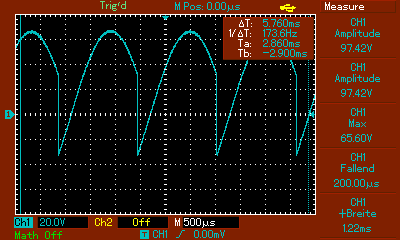
\includegraphics[width=\textwidth]{images/2_0.png}
        \caption{$\varphi = \SI{0}{\degree}$}
        \label{fig:2_0}
    \end{subfigure}
    \begin{subfigure}{0.3\textwidth}
        \centering
        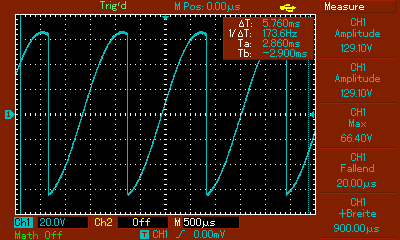
\includegraphics[width=\textwidth]{images/2_45.png}
        \caption{$\varphi = \SI{45}{\degree}$}
        \label{fig:2_45}
    \end{subfigure}
    \begin{subfigure}{0.3\textwidth}
        \centering
        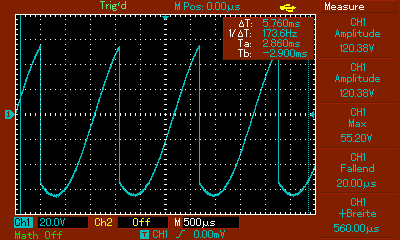
\includegraphics[width=\textwidth]{images/2_90.png}
        \caption{$\varphi = \SI{90}{\degree}$}
        \label{fig:2_90}
    \end{subfigure}
    \par\medskip % Vertikaler Platz
    \begin{subfigure}{0.3\textwidth}
        \centering
        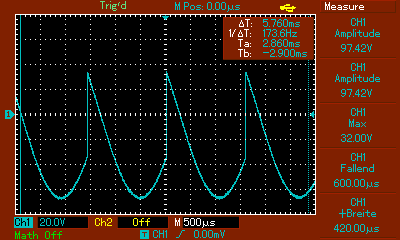
\includegraphics[width=\textwidth]{images/2_180.png}
        \caption{$\varphi = \SI{180}{\degree}$}
        \label{fig:2_180}
    \end{subfigure}
    \begin{subfigure}{0.3\textwidth}
        \centering
        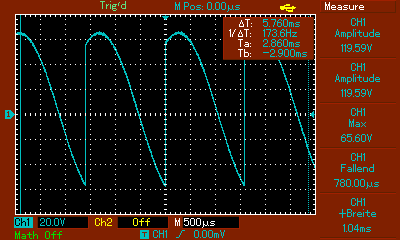
\includegraphics[width=\textwidth]{images/2_270.png}
        \caption{$\varphi = \SI{270}{\degree}$}
        \label{fig:2_270}
    \end{subfigure}
    \caption{Screenshots der Spannung mit zwischengeschaltetem Noise-Generator bei verschiedenen Phasenverschiebungen $\varphi$}
    \label{fig:2}
\end{figure}

In \autoref{tab:phase} sind die Messergebnisse der Spannungsmessung hinter dem Tiefpassfilter gelistet.
$U$ entspricht hier der Messung bei überbrücktem Noise-Generator und für $U_\text{Noise}$ ist dieser zwischengeschaltet.

\begin{table}
    \centering
    \begin{tabular}{S[table-format=3.0] S[table-format=-1.1] S[table-format=-1.1]}
        \toprule
        \tableSI{\varphi}{\degree} & \tableSI{U}{\volt} & \tableSI{U_\text{Noise}}{\volt} \\
        \midrule
        0 & 3.5 & -9.8 \\
        30 & 4.2 & -8.3 \\
        60 & 3.5 & -3.5 \\
        90 & 2.4 & -0.7 \\
        120 & 0.5 & 2.2 \\
        150 & -2.3 & 7.1 \\
        180 & -3.5 & 9.8 \\
        210 & -4.2 & 8.3 \\
        240 & -3.6 & 3.6 \\
        270 & -2.4 & 0.7 \\
        300 & -0.6 & -2.0 \\
        330 & 2.1 & -7.0 \\
        360 & 3.5 & -9.8 \\
        \bottomrule
    \end{tabular}
    \caption{Messergebnisse der Spannungsmessung hinter dem Tiefpassfilter}
    \label{tab:phase}
\end{table}

Mithilfe dieser Messwerte wird jeweils ein Plot erstellt.
Dann wird mithilfe von der Python Bibliothek SciPy und der Funktion curve\_fit jeweils eine Ausgleichskurve erstellt.\cite{scipy}

Hierfür wird nach \autoref{eq:u_out} die Gleichung
\begin{equation}
    U = \frac{2}{\pi}  a \cos(\varphi+b)
\end{equation}
mit den Parametern $a$ und $b$ verwendet.

Damit ergeben sich die Parameter
\begin{align*}
    a =& \SI{6.6+-0.1}{\volt} \\
    b =& \SI{-33+-1}{\degree} \\
    a_\text{Noise} =& \SI{-13.9+-0.7}{\volt} \\
    b_\text{Noise} =& \SI{-5+-3}{\degree}.
\end{align*}
Die entsprechenden Plots sind in \autoref{fig:plot_phase} und in \autoref{fig:plot_phase_noise} zu sehen.

\begin{figure}
    \centering
    \includegraphics[width=\textwidth]{build/plot_phase.pdf}
    \caption{Plot der Spannung bei nicht zwischengeschaltetem Noise-Generator}
    \label{fig:plot_phase}
\end{figure}

\begin{figure}
    \centering
    \includegraphics[width=\textwidth]{build/plot_phase_noise.pdf}
    \caption{Plot der Spannung bei zwischengeschaltetem Noise-Generator}
    \label{fig:plot_phase_noise}
\end{figure}

\subsection{Untersuchung der Lichtdetektion mit dem Lock-In Verstärker}

Wie in \autoref{sec:Durchführung} beschrieben, wurde die Spannung einer Photodiode über den Lock-In Verstärker gemessen. 
In \autoref{tab:led} sind die entsprechenden Messergebnisse gelistet.

\begin{table}
    \centering
    \begin{tabular}{S[table-format=2.0] S[table-format=-1.1]}
        \toprule
        \tableSI{r}{\centi\meter} & \tableSI{U}{\volt} \\
        \midrule
        4 & -3.2 \\
        6 & -3.4 \\
        8 & -3.5 \\
        10 & -3.5 \\
        12 & -3.6 \\
        14 & -3.5 \\
        16 & -3.0 \\
        18 & -2.5 \\
        \bottomrule
    \end{tabular}
        \begin{tabular}{S[table-format=2.0] S[table-format=-1.1]}
            \toprule
            \tableSI{r}{\centi\meter} & \tableSI{U}{\volt} \\
            \midrule
        20 & -2.4 \\
        22 & -1.9 \\
        24 & -1.6 \\
        26 & -1.5 \\
        28 & -1.3 \\
        30 & -1.2 \\
        & \\
        & \\
        \bottomrule
    \end{tabular}
    \caption{Messergebnisse der Lichtintensitätsabnahme}
    \label{tab:led}
\end{table}

Auch diese Messergebnisse sind in einem Plot (\autoref{fig:plot_led}) dargestellt.

Die Ausgleichskurve wird mit 
\begin{equation}
    U = \frac{a}{r^2} + b
\end{equation}
bestimmt. Da schon an den Werten in \autoref{tab:led} zu sehen ist, dass die Werte von $r =$ \SIrange{4}{12}{\centi\meter} nicht mit $1/r^2$ abfallen,
werden für die Ausgleichsrechnung nur die Werte von $r =$ \SIrange{14}{30}{\centi\meter} verwendet.
Dadurch ergeben sich die Parameter
\begin{align*}
    a =& \SI{0.059+-0.004}{\volt\meter\squared} \\
    b =& \SI{0.6+-0.1}{\volt}.
\end{align*}

\begin{figure}
    \centering
    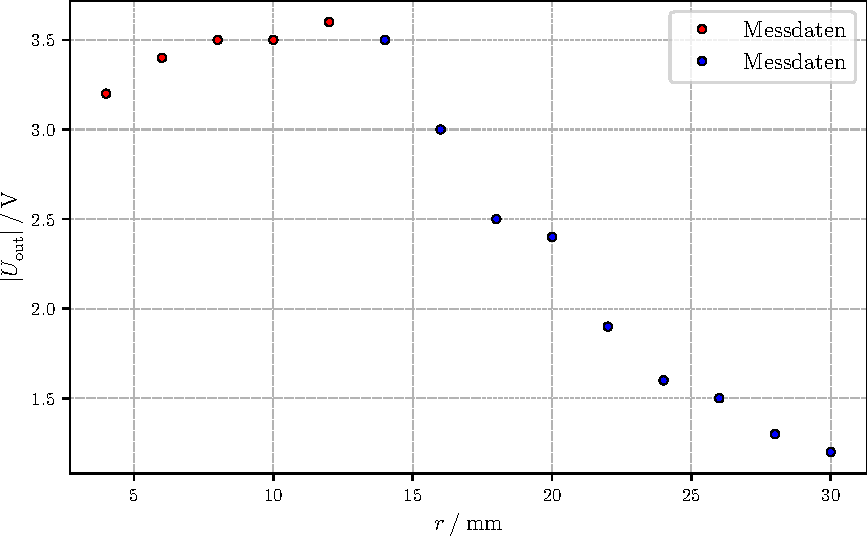
\includegraphics[width=\textwidth]{build/plot_led.pdf}
    \caption{Plot der Daten aus \autoref{tab:led}}
    \label{fig:plot_led}
\end{figure}

Als maximale Distanz, bei der die Lichtintensität noch gemessen werden konnte, wurde ungefähr $r=\SI{80}{\centi\meter}$ beobachtet.